% !TEX root = ../main.tex

\chapter{Action plan}
\label{chp:action_plan}

Making and following an action plan is a learning curve. The first hurdle to take is setting a clear goal, in other words determining the result of the practical study during the internship.  Once the search topic and title of this thesis was decided and approved, making an operational action plan is the next challenge. Defining the strategy and intermediate steps is necessary to achieve the set goals, followed by determining the order and timing for each of these intermediate steps.

From the beginning it was clear that an excessive exploratory study is necessary to create a good foundation to build the technical development on. 

After investigating how a search experience for a website that shows information to help decide between libraries, this experience needs to be set up. The package manager in question is Yarn. Setting up a development environment on the Yarn website is a section of getting to know React InstantSearch in depth. All this was done during the first 4 weeks of the internship.

In the second month the accent was on switching to React InstantSearch in Yarn combined with making a prototype of framework-agnostic InstantSearch. During this stage the found solutions were compared. 

The next step is to integrate multiple frameworks with the connector-based library and presenting this PoC framework integration with full widgets.

During the fourth and last month work was done on documenting solutions and incorporating detail pages in the yarn website.

Reflection, modifying and anchoring was done during the whole process. Following the action plan was not easy. Due to unforeseen circumstances it was necessary to keep a flexible approach to this plan.

\begin{figure}
  \centering
  \includegraphics[width=\textwidth, height=0.95\textheight, keepaspectratio]{action-plan-gantt.pdf}
\end{figure}

\newpage

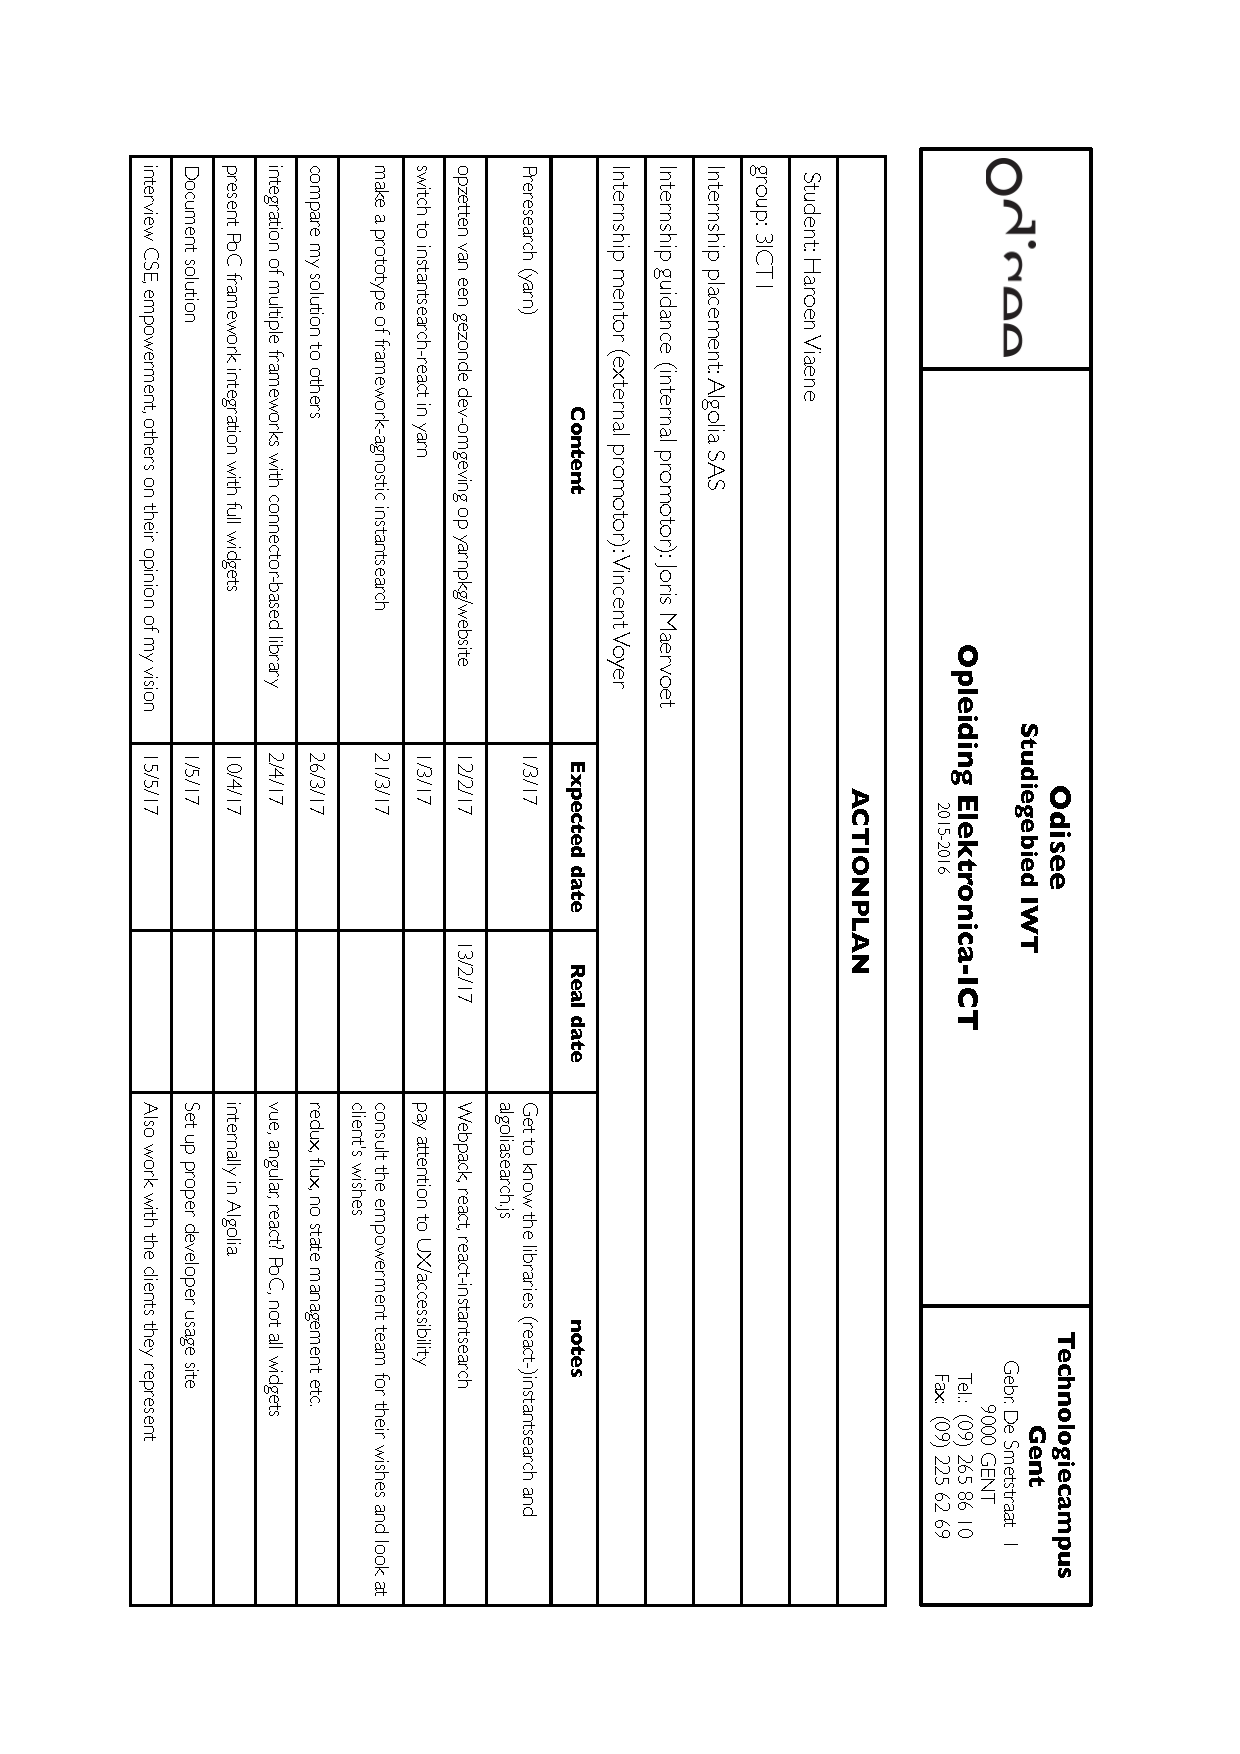
\includegraphics[width=\textwidth, height=0.95\textheight, keepaspectratio]{action-plan.pdf}
